\subsection{Solving the DE}
We can solve these differential equation through separation of variables:

\textbf{Case 1: }
From 1 we have:

\begin{align*}
    -kv^2 &= m \frac{dv}{dt}
    \\ \int \frac{1}{v^2} dv &= \int \frac{-k}{m} dt
    \\ -\frac{1}{v} + c_1 &= \frac{-kt}{m}
    \\ -\frac{m}{v} + c_{1}m &= -kt
    \\ -\frac{m}{v} + c_{1}m + kt &=0
    \\ \frac{m}{v} &= c_{1}m + kt
    \\ \frac{v}{m} &= \frac{1}{c_{1}m+kt}
    \\ \Aboxed{v &= \frac{m}{c_{1}m+kt}}
\end{align*}

\textbf{Case 2:}
From 2 we have: 

\begin{align*}
    -kv^2 - F_b &= m \frac{dv}{dt}
    \\ \int \frac{1}{kv^2 + F_b} dv &= \int -\frac{1}{m} dt
    \\  \int \frac{1}{\frac{k}{F_b}v^2 + 1} dv &= \int -\frac{F_b}{m} dt
    \\ \sqrt{\frac{F_b}{k}} \arctan{(v\sqrt{\frac{k}{F_b}})} &= -\frac{F_b}{m}t + c_2
    \\ \Aboxed{\sqrt{\frac{k}{F_b}} \arctan{(v\sqrt{\frac{k}{F_b}})} &= -\frac{k}{m}t + c_2}
\end{align*}

\subsection{Solutions of the DE}
\textbf{Case1: } 
Using the initial conditions, we can find v as a function of t
\\ \\
Using the point (t=0, v=96), we see that:
\begin{center}
\begin{align*}
    v &= \frac{m}{kt+cm}
    \\ 96 &= \frac{1}{c_1}
    \\ c &= \frac{1}{96}
\end{align*}
\end{center}
Using the point (t=9, v=55), we see that:
\begin{center}
\begin{align*}
    v &= \frac{m}{kt+c_1m}
    \\ 55 &= \frac{m}{9k + c_1m} = \frac{96m}{864k + m} && \text{As $c=\frac{1}{96}$}
    \\ 864k &= \frac{96}{55}m - m
    \\ k &= \frac{1}{864}(\frac{96}{55}m - m)
    \\ &= \text{103.535 $N/ms^{-1}$}
\end{align*}
\end{center}

From this we can deduce that for case 1:
\begin{center}
\begin{align*}
    v &= \frac{m}{kt+c_{1}m}
    \\ v &= \frac{1}{\frac{k}{m}t+\frac{1}{96}}
    \\ \Aboxed{v &= \frac{96}{0.0828t + 1}}
\end{align*}
\end{center}

\textbf{Case 2: } 
Using the initial conditions, we can find v as a function of t
\\ \\
Using the point (t=26, v=0), we see that:
\begin{center}
\begin{align*}
    \sqrt{\frac{k}{F_b}} \arctan{(v\sqrt{\frac{k}{F_b}})} &= -\frac{k}{m}t + c_2
    \\ -\frac{26k}{m} + c_2 &= 0
    \\ c_2 &= \frac{26k}{m} 
    \\ &= 0.02243
\end{align*}
\end{center}
This means our equation now becomes:
\begin{equation}
    \sqrt{\frac{k}{F_b}} \arctan{(v\sqrt{\frac{k}{F_b}})} = -\frac{k}{m}t + 0.02243
\end{equation}
\\ \\
Using the point (t=9, v=55), we see that:
\\
\begin{center}
\begin{align*}
    \sqrt{\frac{k}{F_b}} \arctan{(v\sqrt{\frac{k}{F_b}})} &= -\frac{k}{m}t + 0.02243
    \\ \sqrt{\frac{k}{F_b}} \arctan{(55\sqrt{\frac{k}{F_b}})} &= -9\frac{k}{m} + 0.02243
\end{align*}
\end{center}
To find $F_b$, we can use Newton-Raphson, by letting $\alpha=\sqrt{\frac{k}{F_b}}$ and substituting $9 \frac{k}{m} = 7.764\times{10^{-3}}$
\begin{align*}
    \alpha \arctan{(55\alpha)} &= -9 \frac{k}{m} + 0.02243
\end{align*}
\begin{equation}
    \alpha \arctan{(55\alpha)} - 0.014665 = 0
\end{equation}
Thus by applying Newton-raphson on the above equation, we will be able to find alpha, giving us a value for $F_b$

\subsection{Using Newton-Raphson to find $\alpha$}
\begin{align*}
    \text{let } f(\alpha) &= \alpha \arctan{(55\alpha)} - 0.014665
    \\ \text{Therefore } f'(\alpha) &= \arctan{55a} + \frac{55\alpha}{1+3025\alpha^2}
\end{align*}

\begin{figure}[H]
\centering

\begin{tikzpicture}
\begin{axis}[
    %axis lines = left,
    xlabel = x,
    ylabel = $f(x)$,
]
%Below the red parabola is defined
\addplot [
    domain=0:0.02,
    samples=100, 
    color=red,
]{x*rad(atan(55*x))-0.01463};
\addlegendentry{$xatan{55x}-0.01463$}
\end{axis}
\end{tikzpicture}
\caption{Graph showing the graph of $f(x)$}
\end{figure}

Using the graph of $f(x)$, we see that the root is close to 0.02. Therefore we will use 0.02 as our inital guess for the root.
\\ \\
Using the iterative formula, $x_{i+1} := x_{i}-\frac{f(x)}{f'(x)}$, to find the next closest root we can produce a table showing all the iterations and the next approximation of the root it gave.


\begin{table}[h]
\centering
    \begin{tabular}{|l|l|l|l|l|}
        \hline
        i & $x_i$ & $f(x)$ & $f'(x)$ & $x_{i+1}$ \\ \cline{1-5}
        1 & 0.02000 & 0.00203 & 1.33072 & 0.01847 \\ \cline{1-5}
        2 & 0.01847 & 0.00003 & 1.29333 & 0.01845 \\ \cline{1-5}
        3 & 0.01845 & 0.00000 & 1.29276 & 0.01845 \\ \cline{1-5}
    \end{tabular}
    \caption{Newton Raphson Iterations}
\end{table}
\
Thus we find that alpha is 0.01845, meaning that the fraction \\ $\sqrt{\frac{k}{F_b}} = 0.01845$ to 5dp.
\newline \newline
Therefore by rearranging for v, we can conclude that for case 2:
\begin{align*}
    \alpha \arctan{(\alpha v)} &= -\frac{k}{m}t + 0.02243
    \\ \arctan{(\alpha v)} &= -\frac{k}{m\alpha}t + \frac{0.02243}{\alpha}
    \\ v &= \frac{1}{\alpha} \tan{(-\frac{k}{m\alpha}t + \frac{0.02243}{\alpha})}
    \\ \Aboxed{v &=  54.2\tan{(-0.0468t + 1.22)}}
\end{align*}

\subsection{Model Performance}

\begin{table}[H]
\centering
    \begin{tabular}{|l|l|l|l|l|l|l|l|l|l|l|l|l|l|l|l|l|}
        \hline
        t(s) & 0 & 1 & 2 & 3 & 4 & 5 & 6 & 7 & 8 & 9 \\ \cline{1-11} 
        predicted v(m/s) & 96.00 & 88.66 & 82.36 & 76.90 & 72.12 & 67.89 & 64.14 & 60.77 & 57.75 & 55.01
        \\ \cline{1-11}
        Actual v(m/s) & 96 & 89 & 82 & 77 & 72 & 68 & 64 & 61 & 58 & 55 \\ \cline{1-11}
        $d^2$ & 0.000 & 0.116 & 0.130 & 0.010 & 0.013 & 0.012 & 0.019 & 0.051 & 0.064 & 0.000 \\ \cline{1-11}
    \end{tabular}
    \caption{Case 1}
    \vspace{0.5cm}

    \begin{tabular}{|l|l|l|l|l|l|l|l|l|l|l|l|}
        \hline
        t(s) & 10 & 11 & 12 & 13 & 14 & 15 & 16 & 17 & 18 \\ \cline{1-10}
        predicted v(m/s) & 50.70 & 46.14 & 41.93 & 38.01 & 34.34 & 30.89 & 27.61 & 24.49 & 21.50 \\ \cline{1-10}
        Actual v(m/s) & 50 & 46 & 41 & 38 & 34 & 31 & 27 & 24 & 21 \\ \cline{1-10}
        $d^2$ & 0.484 & 0.018 & 0.858 & 0.000 & 0.118 & 0.012 & 0.377 & 0.241 & 0.247 \\ \cline{1-10}
    \end{tabular}
    \caption{Case 2}
    \vspace{0.5cm}
    
    \begin{tabular}{|l|l|l|l|l|l|l|l|l|}
        \hline
        t(s) & 19 & 20 & 21 & 22 & 23 & 24 & 25 & 26 \\ \cline{1-9}
        predicted v(m/s) & 18.61 & 15.82 & 13.10 & 10.45 & 7.84 & 5.26 & 2.71 & 0.17 \\ \cline{1-9}
        Actual v(m/s) & 18 & 16 & 13 & 10 & 8 & 5 & 3 & 0
        \\ \cline{1-9}
        $d^2$ & 0.376 & 0.032 & 0.011 & 0.199 & 0.027 & 0.069 & 0.083 & 0.030 \\ \cline{1-9}
    \end{tabular}
    \caption{Case 2 continued}
    \vspace{0.5cm}
\end{table}

\begin{figure}[H]
\centering
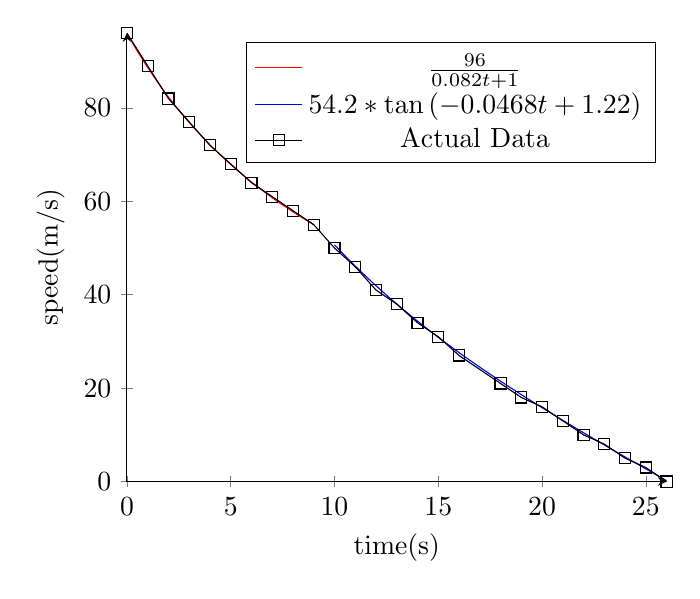
\begin{tikzpicture}
\begin{axis}[
    axis lines = left,
    xlabel = time(s),
    ylabel = speed(m/s),
]
%Below the red parabola is defined
\addplot [
    domain=0:9,
    samples=100, 
    color=red,
]
{96/(0.0828*x + 1)};
\addlegendentry{$\frac{96}{0.082t + 1}$}
%Here the blue parabloa is defined
\addplot [
    domain=10:26, 
    samples=100, 
    color=blue,
    ]
    {54.2*tan((1.22-0.0468*x)*(180/3.1415))};
\addlegendentry{$54.2*\tan{(-0.0468t+1.22)}$}
 
 \addplot[
    color=black,
    mark=square]
    coordinates {(0,96)(1,89)(2,82)(3,77)(4,72)(5,68)(6,64)(7,61)(8,58)(9,55)(10,50)(11,46)(12,41)(13,38)(14,34)(15,31)(16,27)(18,21)(19,18)(20,16)(21,13)(22,10)(23,8)(24,5)(25,3)(26,0)};
\addlegendentry{Actual Data}
\end{axis}
\end{tikzpicture}
\caption{Graph showing the predicted velocity values against the actual velocity values}
\end{figure}
